
%(BEGIN_QUESTION)
% Copyright 2009, Tony R. Kuphaldt, released under the Creative Commons Attribution License (v 1.0)
% This means you may do almost anything with this work of mine, so long as you give me proper credit

In instrumentation parlance, a {\it transducer} is a calibrated device used to convert one standardized signal into another standardized signal.  One very common form of transducer is an {\it I/P transducer}, which converts an electric current signal into a pneumatic pressure signal:

$$\includegraphics[width=15.5cm]{i00084x01.eps}$$

The symbols shown above are standard for process and instrumentation diagrams (P\&ID's), where an electric cable is shown as a dashed line, a pneumatic pipe or tube shown as a line with double hash-marks periodically drawn through it, and the instrument is a circle with letters (in this case, ``Y'', representing a signal relay, computing element, transducer, or converter).

The most popular range for electric current signals is 4 to 20 mA DC.  The most common range for pneumatic (air pressure) signals is 3 to 15 PSI.  Therefore, the most common type of I/P transducer has an input range of 4-20 mA and an output range of 3-15 PSI.  Both of these ranges are there to represent some measured or manipulated quantity in an instrument system.  That is, 0\% of range will be represented by a 4 mA input signal to the I/P, and a 3 PSI output signal; 100\% of range will be represented by a 20 mA input signal and a 15 PSI output signal; 50\% range will be represented by a 12 mA input and a 9 PSI output.

Complete all the missing data in the following calibration table for this I/P transducer, and then describe how you were able to correlate the different percentages of range with specific current and pressure signal values:

% No blank lines allowed between lines of an \halign structure!
% I use comments (%) instead, so that TeX doesn't choke.

$$\vbox{\offinterlineskip
\halign{\strut
\vrule \quad\hfil # \ \hfil & 
\vrule \quad\hfil # \ \hfil & 
\vrule \quad\hfil # \ \hfil \vrule \cr
\noalign{\hrule}
%
% First row
Input current & Percent of range & Output pressure \cr
%
% Another row
(mA) & (\%) & (PSI) \cr
%
\noalign{\hrule}
%
% Another row
4 & 0 & 3 \cr
%
\noalign{\hrule}
%
% Another row
 & 10 &  \cr
%
\noalign{\hrule}
%
% Another row
 & 20 &  \cr
%
\noalign{\hrule}
%
% Another row
 & 25 &  \cr
%
\noalign{\hrule}
%
% Another row
 & 30 &  \cr
%
\noalign{\hrule}
%
% Another row
 & 40 &  \cr
%
\noalign{\hrule}
%
% Another row
12 & 50 & 9 \cr
%
\noalign{\hrule}
%
% Another row
 & 60 &  \cr
%
\noalign{\hrule}
%
% Another row
 & 70 &  \cr
%
\noalign{\hrule}
%
% Another row
 & 75 &  \cr
%
\noalign{\hrule}
%
% Another row
 & 80 &  \cr
%
\noalign{\hrule}
%
% Another row
 & 90 &  \cr
%
\noalign{\hrule}
%
% Another row
20 & 100 & 15 \cr
%
\noalign{\hrule}
} % End of \halign 
}$$ % End of \vbox

Challenge: build a computer spreadsheet that calculates all current and pressure values from given percentages.

\underbar{file i00084}
%(END_QUESTION)





%(BEGIN_ANSWER)

$$\vbox{\offinterlineskip
\halign{\strut
\vrule \quad\hfil # \ \hfil & 
\vrule \quad\hfil # \ \hfil & 
\vrule \quad\hfil # \ \hfil \vrule \cr
\noalign{\hrule}
%
% First row
Input current & Percent of range & Output pressure \cr
%
% Another row
(mA) & (\%) & (PSI) \cr
%
\noalign{\hrule}
%
% Another row
4 & 0 & 3 \cr
%
\noalign{\hrule}
%
% Another row
5.6 & 10 & 4.2 \cr
%
\noalign{\hrule}
%
% Another row
7.2 & 20 & 5.4 \cr
%
\noalign{\hrule}
%
% Another row
8 & 25 & 6 \cr
%
\noalign{\hrule}
%
% Another row
8.8 & 30 & 6.6 \cr
%
\noalign{\hrule}
%
% Another row
10.4 & 40 & 7.8 \cr
%
\noalign{\hrule}
%
% Another row
12 & 50 & 9 \cr
%
\noalign{\hrule}
%
% Another row
13.6 & 60 & 10.2 \cr
%
\noalign{\hrule}
%
% Another row
15.2 & 70 & 11.4 \cr
%
\noalign{\hrule}
%
% Another row
16 & 75 & 12 \cr
%
\noalign{\hrule}
%
% Another row
16.8 & 80 & 12.6 \cr
%
\noalign{\hrule}
%
% Another row
18.4 & 90 & 13.8 \cr
%
\noalign{\hrule}
%
% Another row
20 & 100 & 15 \cr
%
\noalign{\hrule}
} % End of \halign 
}$$ % End of \vbox

\vskip 10pt

Follow-up question: explain the procedure for starting with a current value in milliamps and calculating the equivalent percentage.

%(END_ANSWER)





%(BEGIN_NOTES)

Here are the equations I used to arrive at my answers:

$$\hbox{current} = (16 \hbox{ mA}) \left( {\% \over 100}\right) + (4 \hbox{ mA})$$

$$\hbox{pressure} = (12 \hbox{ PSI}) \left( {\% \over 100}\right) + (3 \hbox{ PSI})$$

In general, to go from a percentage value to either current or pressure, take that percentage (as a decimal value between 0 and 1 inclusive) and multiply it by the {\it span} of the signal range, then add the live zero offset.

\vskip 10pt

Going from either a current value or a pressure value to a percentage is little more than the reverse of the above procedure.  Watch how I convert a current value of 16.8 milliamps into a percentage of range:

$$16.8 \hbox{ mA} - 4.0 \hbox{ mA} = 12.8 \hbox{ mA} \hskip 50pt \hbox{\it First, subtract the live-zero offset}$$

$${12.8 \hbox{ mA} \over 16.0 \hbox{ mA}} = 0.8 \hskip 50pt \hbox{\it Second, divide that number by the span}$$

$$0.8 \times 100\% = 80\% \hskip 50pt \hbox{\it Finally, convert this into a percentage}$$

These sorts of calculations are done quite often by instrument technicians as they troubleshoot instrument systems.  Imagine troubleshooting a 4-20 mA instrument circuit using an ammeter to measure current.  How do you correlate the measured current value into a percentage of range, and from that into an equivalent process measurement?  These calculations allow you to do this, which gives you a way to translate the current signals you measure with your meter into equivalent process values, without having to look at a pre-calibrated indicator.


%INDEX% Basics, transmitter: input and output ranges
%INDEX% Calibration: table, I/P transducer

%(END_NOTES)


